%!TEX root = nips2015.tex
\section{Results}

We tested out different configurations of the experiments mentioned in the last section and evaluated them using the difference in scores of the network and GnuGo. We expected that, as the network improved its tactics, the changes would manifest in the GnuGo opponent having more difficulty scoring higher points thus increasing the difference from negative to positive.

\begin{figure}[h!]
\centering
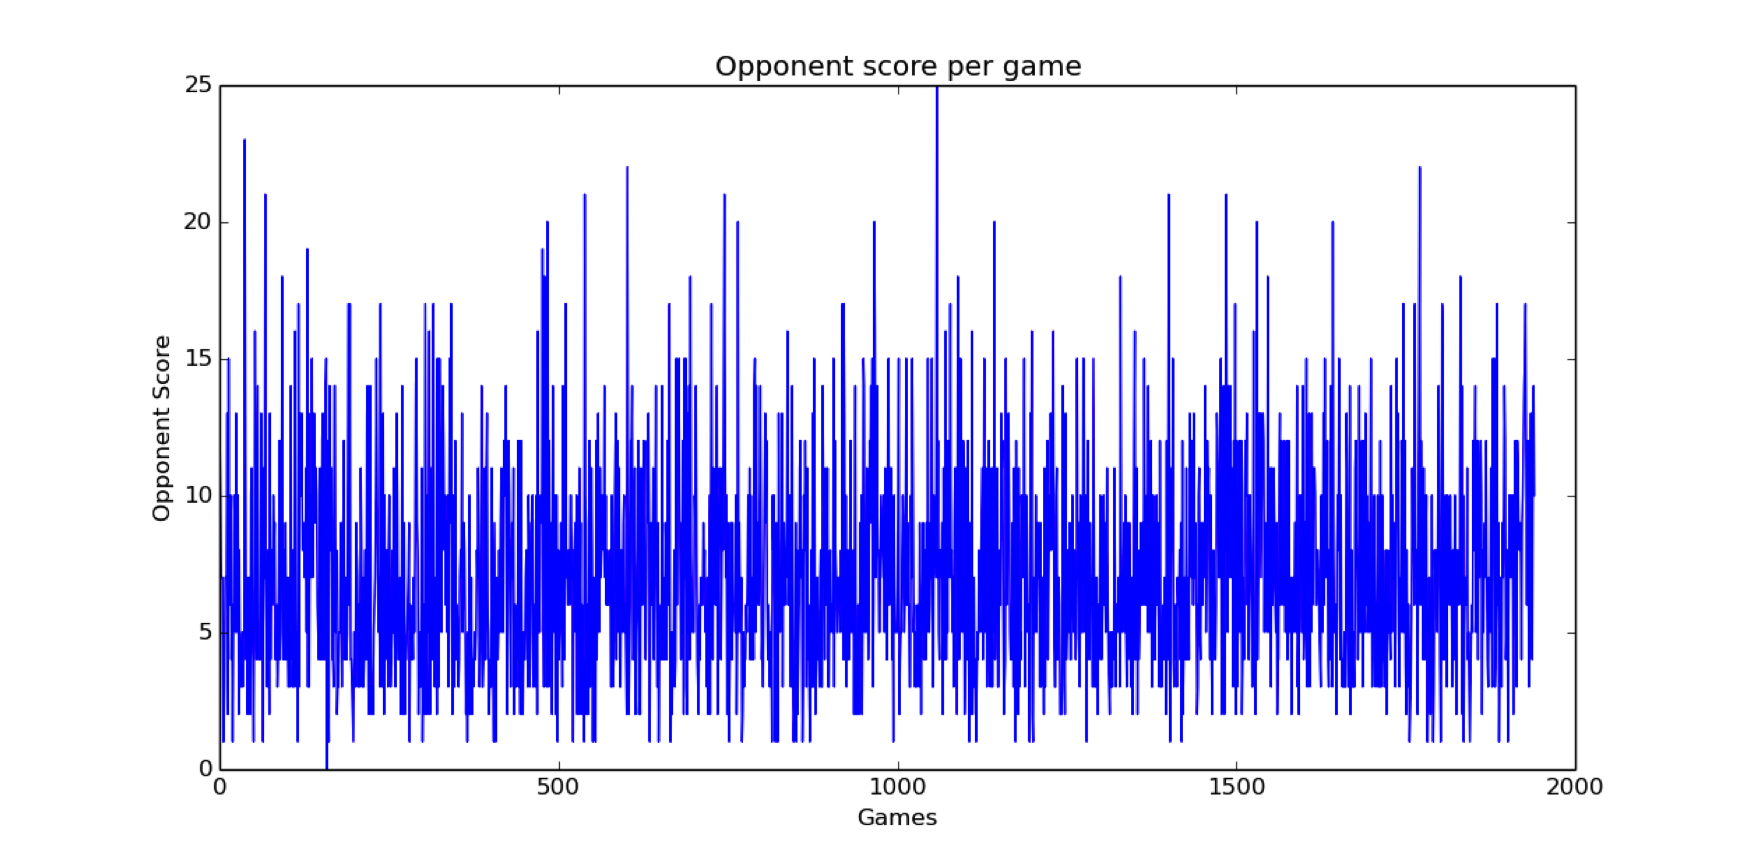
\includegraphics[scale=0.5]{training_score.png}
\caption{Opponent (GnuGo) score per game on a 7 $\times$ 7 board. The network was provided with a 7 layer input and consisted of 5 convolution layers}
\label{fig:score}
\end{figure}


Unfortunately, in all cases we were unable to get consistent performance, regardless of specific parameter settings. It did win occasionally, but overall GnuGo beat the network consistently. In the games which it won, we could not make out a clear strategy so we attribute the wins to chance. Figure \ref{fig:score} shows one particular training session that we allowed to run for 2000 games. 

\section{Analysis and Future Work}
In this section, we offer hypotheses that attempt to explain why our agent was not able to learn an appropriate Q-network for Go. First, we simply could not generate a sufficient number of quality training examples. A large number of our training examples were illegal moves with a reward of -1. Even if we disregard this, the speed with which we were able to generate training examples was simply far from sufficient. Considering that [2] trained on 16 million examples, and that, assuming approximately 50 moves per game on a board of size 7, it took us 3 days to generate 100,000 examples, it is simply infeasible to expect to generate a data set of comparable size. We must then rely on using training examples in a more efficient way, or we must avoid training a network from scratch.

As mentioned before, weight tying is one way to use training examples more efficiently, and initializing the Q-network to a DCNN would definitely help with avoiding illegal moves. Still, weight tying only offers an improvement of an approximate factor of 8. We can think of this as allowing us to generate 800,000 moves in 3 days, which is still far from satisfactory. While it might not be sufficient, implementing weight-tying can undeniably help in training the Q-network, and is a good direction for future work.

Additionally, it might very well be completely necessary to use a combination approach involving Monte-Carlo and convolutional networks, as recent results indicate. 

While we have not been able to train a Q-network, we believe that we have still made a contribution to the community with our code. As of now, anyone can download our code from github and quickly experiment with their own modifications to the Q-network or other modules. Just as the open source ALE environment allowed DeepMind to test their system, our code will allow others in the community to test their strategies on Go.